\documentclass[11pt, letterpaper]{article}
\usepackage[utf8]{inputenc}
\usepackage[margin=1in]{geometry}
\usepackage{enumitem}
\usepackage{indentfirst}
\usepackage{titling}
\usepackage{graphicx}
\usepackage{amsmath}
\usepackage{amsfonts}
\usepackage{amsthm}
\usepackage{mathtools}
\usepackage{hyperref}
\usepackage{mathabx}
\usepackage{caption}
%\usepackage{subcaption}
\usepackage{bm}
\usepackage{textcomp}
\usepackage{subfig}
\usepackage[dvipsnames]{xcolor}
\graphicspath{ {./} }
\DeclareMathAlphabet{\altmathcal}{OMS}{cmsy}{m}{n}

\newtheorem{theorem}{Theorem}[subsection]
\newtheorem{corollary}{Corollary}[theorem]
\newtheorem{lemma}[theorem]{Lemma}

\theoremstyle{definition}
\newtheorem{definition}{Definition}[subsection]

\theoremstyle{remark}
\newtheorem*{remark}{Remark}

\newcommand{\bv}[2][]{\bm{\vec{#2}_{#1}}}

\setlength{\parindent}{0cm}
\setlength{\parskip}{1em}
\renewcommand{\baselinestretch}{1.5}

\hypersetup{
    colorlinks=true,
    linkcolor=cyan,
    filecolor=magenta,      
    urlcolor=blue,
}

\title{Chapter IX: Sources of Magnetic Fields}
\author{Chenyi Zhu}
\date{July 7th, 2020}

\begin{document}


\begin{titlingpage}
	\maketitle
	
	\begin{figure}[h!]
		\centering
		
	\end{figure}
		
\end{titlingpage}

\section{Introduction.}\label{sec:intro}
We have seen that a charged object produces an electric field $\bv{E}$ at all points in space. Similarly, a magnet is a source of a magnetic field $\bv{B}$, which you can show by moving it close to a magnet. Magnets consist of two poles, the north and the south. However, unlike electric charges which can be isolated, magnetic poles always come in a pair. Breaking the bar magnet results in two new bar magnets, each with a north and south pole. Magnetic monopoles do not exist in isolation, but are of theoretical interests. We cannot define magnetic field $\bv{B}$ the same way as the electric field $bv{E}$ \[\bv{E} = \frac{\bv[e]{F}}{q}\] due to the lack of magnetic monopoles. 

\section{Definition of Magnetic Fields.}\label{sec:def}
To define the magnetic field at a point, consider a particle of charge $q$ and moving at a velocity $\bv{v}$. From experimental data we have the following observations:
\begin{itemize}
	\item The magnitude of the magnetic force $\bv[B]{F}$ exerted on the charged particle is proportional to both $\bv{v}$ and $q$;
	\item The magnitude and direction of $\bv[B]{F}$ depends on $\bv{v}$ and $\bv{B}$;
	\item The magnetic force $\bv[B]{F}$ vanishes when $\bv{v}$ is parallel to $\bv{B}$. However, when $\bv{v}$ makes an angle $\theta$ with $\bv{B}$, the direction of $\bv[B]{F}$ is perpendicular to the plane formed by $\bv{v}$ and $\bv{B}$, and the magnitude of $\bv[B]{F}$ is proportional to $\sin{\theta}$;
	\item When the sign of the charge of the particle is switched from positive to negative (or vice versa), the direction of the magnetic force also reverses.
\end{itemize}
All of the above can summarize to one simple expression: 
\begin{equation}\label{eqn:magnetic-force}
	\boxed{\bv[B]{F} = q\bv{v}\times\bv{B}}
\end{equation}
This expression is a working definition of the magnetic field at a point in space. The magnitude $|\bv[B]{F}|$ is then: \[F_B = |q|vB\sin{\theta}\] and the SI unit of magnetic field is the tesla ($T$): \[1\, T = 1\,\frac{N}{C\cdot m/s} = 1\,\frac{N}{A\cdot m}\] Another commonly used non-SI unit for $\bv{B}$ is the gauss ($G$), where $1\, T = 10^4\,G$. 

By convention, for magnetic field lines pointing 

\textbf{Note}: $\bv[B]{F}$ is always perpendicular to $\bv{v}$ and $\bv{B}$, and cannot change the particle's speed $v$ (and thus kinetic energy as well), i.e. magnetic forces cannot speed up or slow down a charged particle. Consequently, $\bv[B]{F}$ can do no work on the particle: \[dW = \bv[B]{F}\cdot\, d\bv{s} = q(\bv{v}\times\bv{B})\cdot\bv{v}\, dt = q(\bv{v}\times\bv{v})\cdot\bv{B}\, dt = 0\] The direction of $\bv{v}$, however, can be altered y the magnetic force, and we shall show that now.

\section{Magnetic Force on a Current-Carrying Wire.}\label{sec:wire}
We have just seen that a charged particle moving through a magnetic field experiences a magnetic force $\bv[B]{F}$. Since electric current consists of a collection of charged particles \textbf{in motion}, when placed in a magnetic field, a current-carrying wire will also experience a magnetic force. Let's look at an example. 

Consider a long straight wire suspended in the region between the two magnetic poles. The magnetic field points out of the page and is represented with dots ($\bullet$, otherwise $\times$). When a downward current passes through, the wire is deflected to the left. However, if we send a current upwards, the wire will be deflected to the right.
\begin{figure}[h!]
		\centering
		\subfloat{{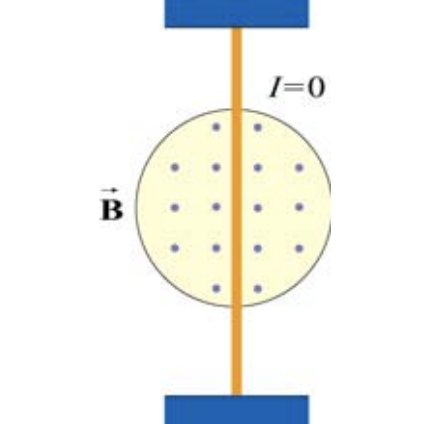
\includegraphics[width=3cm]{middle.png}}}
		\qquad
		\subfloat{{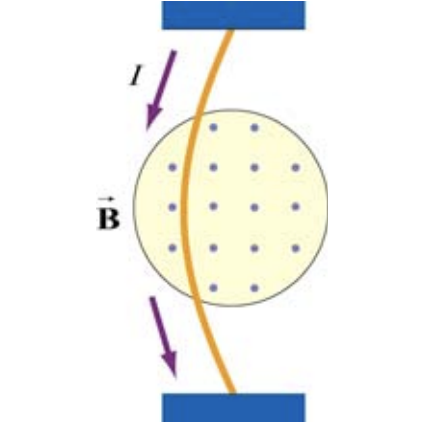
\includegraphics[width=3cm]{left.png}}}
		\qquad
		\subfloat{{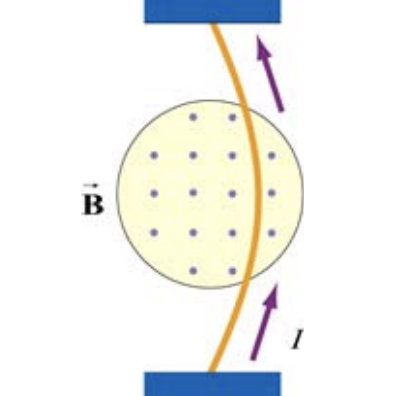
\includegraphics[width=3cm]{right.png}}}
		\caption{Current-carrying wire in a magnetic field.}
\end{figure}

To calculate the force exerted on the wire, consider a segment of wire of length $l$ and cross-sectional area $A$. The magnetic field points into the page. 
\begin{figure}[h!]
	\centering
	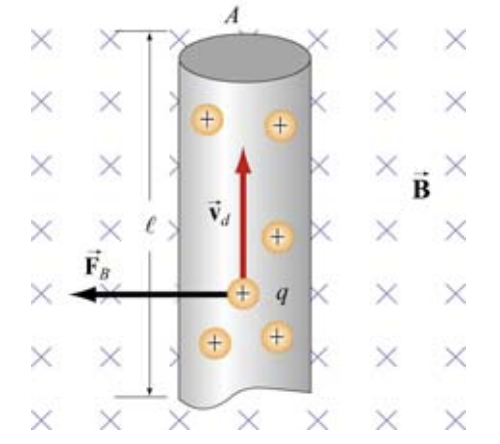
\includegraphics[scale=0.6]{wire}
	\caption{Magnetic force on a conducting wire.}
	\label{fig:wire}
\end{figure}

The charges move at an average drift velocity $\bv[d]{v}$. Since the total amount of charge in this segment is $Q_{tot} = q(nAl)$, where $n$ is the number of charges per unit volume (recall from chapter $5$ section on current density), the total magnetic force on the segment is \[\bv[B]{F} = Q_{tot}\bv[d]{v}\times\bv{B} = qnAl(\bv[d]{v}\times\bv{B}) = I(\bv{l}\times\bv{B})\] where $I = nqv_dA$, and $\bv{l}$ is a \textit{length vector} with a magnitude $l$ and in the direction of the current.

For a wire of arbitrary shape, the magnetic force can be obtained by summing over the forces acting on the small segments that make up the wire. Let the differential segment be denoted as $d\bv{s}$.
\begin{figure}[h!]
	\centering
	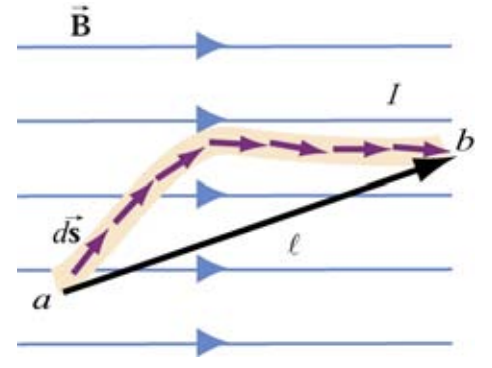
\includegraphics[scale=0.6]{arbitrary}
	\caption{Wire of arbitrary shape in a magnetic field.}
	\label{fig:arbitrary}
\end{figure}

The magnetic force acting on the segment is \[d\bv[B]{F} = Id\bv{s}\times\bv{B}\] and thus the total force is
\begin{equation}\label{eqn:arbitrary}
	\boxed{\bv[B]{F} = I\int_a^b d\bv{s}\times\bv{B}}
\end{equation}
where $a$ and $b$ represent the endpoints of the wire.

For example, with the figure given above, the integral will integrate to the distance (in a straight line) from $a$ to $b$, call it $l$. The magnetic force on the wire would then be given by \[\bv[B]{F} = I\left(\int_a^bd\bv{s}\right)\times\bv{B} = I\bv{l}\times\bv{B}\] Another interesting case arise when the segment above forms a closed loop, in which case \[\bv[B]{F} = I\left(\oint d\bv{s}\right)\times\bv{B} = \bv{0}\] Which tells us that the net magnetic force on a closed loop is $\bv[B]{F} = \bv{0}$. This, however, does not imply that the magnetic field is conservative. See proof \hyperref[subsec:non-conservative]{here}.

\section{Torque on a Current Loop.}\label{sec:loop}
Now we will examine the effect of magnetic fields on current carrying loops. Consider the following scenario:
\begin{figure}[h!]
	\centering
	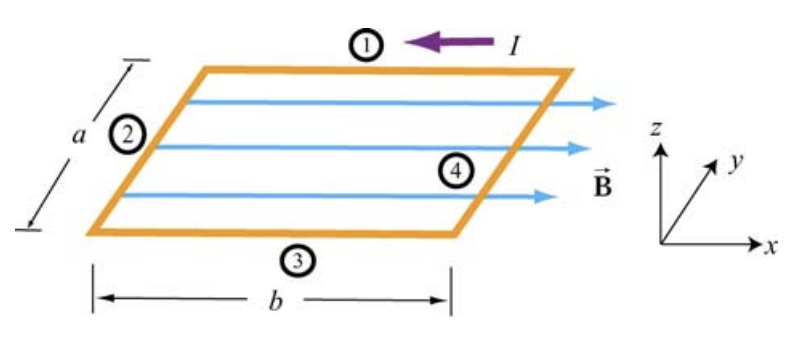
\includegraphics[scale=0.6]{loop_torque}
	\caption{Rectangular current loop in a magnetic field.}
	\label{fig:torque_loop}
\end{figure}

We can immediately eliminate the magnetic forces on sides $1$ and $3$ because their current vectors are parallel/anti-parallel to the field vectors. The non-vanishing forces will act on sides $2$ and $4$, pointing in $\hat{z}$ and -$\hat{z}$ directions respectively, with equal magnitude:
\[
	\left\{
	\begin{array}{@{}ll@{}}
		\bv[2]{F} = I(-a\hat{j})\times (B\hat{i}) = IaB\hat{k}\\
		\bv[4]{F} = I(a\hat{j})\times (B\hat{i}) = -IaB\hat{k}
		
	\end{array}\right.
\]
where $\bv[2]{F}$ is pointing up and $\bv[4]{F}$ down. Thus the net force - sum of all four force vectors acting along each edge of the loop - vanishes. While the force vanishes, torque does not. The forces $\bv[2]{F}$ and $\bv[4]{F}$ produce a torque which will rotate the loop about the $y$-axis. The torque produced with respect to the center of the loop is:
\[
\begin{split}
	\bv{\tau} &= \left(-\frac b2\hat{i}\right)\times \bv[2]{F} + \left(\frac b2\hat{i}\right)\times\bv[4]{F}
				   = \left(-\frac b2\hat{i}\right)\times (IaB\hat{k}) + \left(\frac b2\hat{i}\right)\times (-IaB\hat{k})
				   = IabB\hat{j}\\
				   &= IAB\hat{j}
\end{split}
\]
where $A = ab$ as the area of loop, and positive sign indicates rotation in the clockwise direction. We hence introduce the Area vector $\bv{A} = A\hat{n}$, where $\hat{n}$ is a unit vector normal to the plane of the loop. The default positive direction is determined by the right-hand rule. Therefore, in this case we have $\hat{n} = +\hat{k}$. Rewriting the above answer we have: \[\bv{\tau} = I\bv{A}\times\bv{B}\] in which the torque is maximized when the magnetic field $\bv{B}$ is perpendicular to $\bv{A}$.

Now consider the case where $\bv{A}$ and $\bv{B}$ are separated by angle $\theta$. 
\begin{figure}[h!]
	\centering
	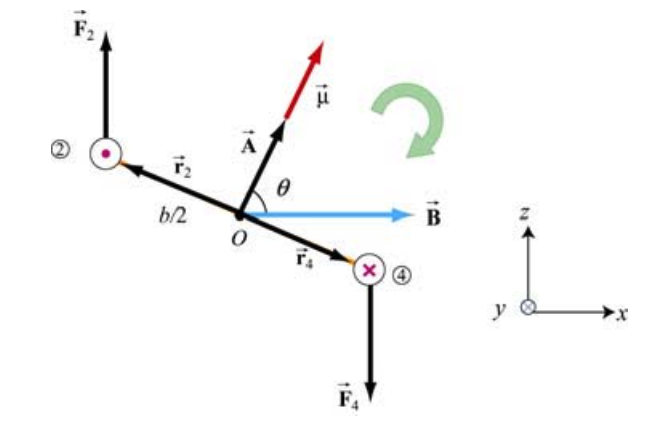
\includegraphics[scale=0.6]{angle}
	\caption{Torque on a current loop.}
	\label{fig:angle}
\end{figure}

The lever arms can be expressed as
\[\bv[2]{r} = \frac b2(-\sin\theta\hat{i} + \cos\theta\hat{k}) = -\bv[4]{r}\]

and the net torque:
\[
\begin{split}
	\bv{\tau} &= \bv[2]{r}\times\bv[2]{F} + \bv[4]{r}\times\bv[4]{F} 
				   = 2\cdot\frac b2(-\sin\theta\hat{i} + \cos\theta\hat{k})\times (IAB\hat{k})
				   = IAB\sin\theta\hat{j}\\
				   &= I\bv{A}\times\bv{B}
\end{split}
\]

For a loop with $N$ turns, the magnitude of torque is \[\tau = NIAB\sin\theta\]
The quantity $NI\bv{A}$ is called the \textbf{magnetic dipole moment} $\bv{\mu}$: 
\begin{equation}\label{eqn: magnetic-dipole-moment}
	\boxed{\bv{\mu} = NI\bv{A}}
\end{equation}

Note that the direction of $\bv{\mu}$ is the same as $\bv{A}$, and its SI unit is ampere-meter$^2$($A\cdot m^2$). We can rewrite the torque as: 
\begin{equation}\label{eqn: torque-dipole}
	\boxed{\bv{\tau} = \bv{\mu} \times \bv{B}}
\end{equation}

This equation is analogous to $\bv{\tau} = \bv{p}\times\bv{E}$, the torque exerted on an electric dipole moment $\bv{p}$ in the presence of an electric field $\bv{E}$. Recall also that the potential energy for an electric dipole is $U = -\bv{p}\cdot\bv{E}$; a similar form applies for a magnetic dipole. External work done to rotate the magnetic dipole from an angle $\theta_0$ to $\theta$ is given by 
\[
\begin{split}
	W_{ext} &= \int_{\theta_0}^{\theta} \tau\, d\theta ^\prime = \int_{\theta_0}^{\theta} (\mu B\sin\theta\prime)\, d\theta\prime = \mu B(\cos\theta_0 - \cos\theta) = \Delta U\\
				&= U - U_0
\end{split}
\]

We know that $W_{ext} = -W$, where $W$ is the work done by the magnetic field. Choosing $U_0 = 0$ at $\theta_0=\pi/2$, the dipole in the presence of an external field then has a potential energy of 
\begin{equation}\label{eqn:magnetic-dipole-energy}
	\boxed{U = -\mu B \cos\theta = -\bv{\mu}\cdot\bv{B}}
\end{equation}

wherein the system is in equilibrium when $\bv{\mu}$ is aligned parallel to $\bv{B}$, making $U$ a minimum with $U_{min} = -\mu B$. On the contrary, when $\bv{mu}$ and $\bv{B}$ are anti-parallel, $U_{max} = \mu B$ is a maximum and the system is most unstable.

\section{Charged Particles in a Uniform Magnetic Field.}\label{sec:particle}
Recall centripetal force: if a particle of mass $m$ moves in a circle of radius $r$ at a constant speed $v$, the particle will experience a radial force of magnitude $F = mv^2/2$ that always points toward the center and is perpendicular to the velocity of the particle. In addition, we have shown in \hyperref[sec:def]{section 2} that the magnetic force $\bv[B]{F}$ is always perpendicular to the velocity $\bv{v}$ of the charged particle and the magnetic field $\bv{B}$. $\bv[b]{F}$ CANNOT do work, it can only change the direction of $\bv{v}$ but not its magnitude. We will now show what happens when a charged particle moves through a uniform magnetic field with its initial velocity $\bv{v}$ at a right angle to $\bv{B}$. Let the charge be $+q$ and the direction of $\bv{B}$ be into the page. In this case, $\bv{B}{F}$ will essentially act as a centripetal force and the particle will move in a circular path in a counterclockwise direction, with \[qvB=\frac{mv^2}{2}\Rightarrow\boxed{r=\frac{mv}{qB}}\]
\begin{figure}[h!]
	\centering
	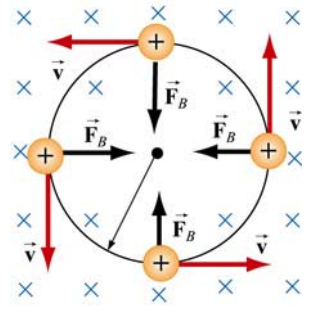
\includegraphics[scale=0.7]{centripetal}
	\caption{Charged particle moving in uniform $\bv{B}$ perpendicular to initial velocity $\bv{v}$.}
	\label{fig:centripetal}
\end{figure}

We can then calculate the period: \[T = \frac{2\pi r}{v} = \frac{2\pi}{v}\frac{mv}{qB} = \frac{2\pi m}{qB}\] and the angular speed $\omega$: \[\boxed{\omega = 2\pi f = \frac{v}{r} = \frac{qB}{m}}\]

If the initial velocity of the charged particle has a component parallel to the magnetic field $\bv{B}$, the resulting trajectory will be a helical path in $3D$ instead of a circle in $2D$.
\begin{figure}[h!]
	\centering
	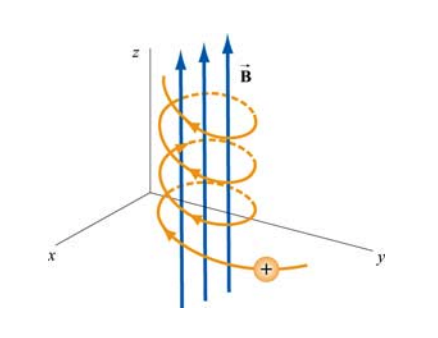
\includegraphics[scale=0.5]{helix}
	\caption{Charged particle moving in helical path.}
	\label{fig:helix}
\end{figure}


\section{Appendix.}
\subsection{Magnetic Fields are Non-conservative}
\label{subsec:non-conservative}
From Wikipedia: A \textit{force field} $\bv{F}$, defined everywhere in space (or within a simply-connected volume of space), is called a \textbf{conservative force} or \textbf{conservative vector field} if it meets any of these three equivalent conditions (for proof of equivalence, see \href{https://en.wikipedia.org/wiki/Conservative_force#Mathematical_description}{here}):
\begin{enumerate}
	\item The curl of $F$ is the zero vector: $\nabla\times\bv{F} = \bv{0}$
	\item There is zero net work done by the force when moving a particle through a trajectory that starts and ends in the same place: $W \equiv \oint_C \bv{F}\cdot\, d\bv{r} = 0$
	\item The force can be written as the negative gradient of a potential, $\Phi$: $\bv{F} = -\nabla\Phi$
\end{enumerate}
The term conservative force comes from the fact that when a conservative force exists, it conserves mechanical energy. The most familiar conservative forces are gravity, the electric force (in a time-independent magnetic field, see Faraday's law), and spring force.

Many forces (particularly those that depend on velocity) are not force fields. In these cases, the three statements above are not equivalent. We have seen that magnetic force satisfies condition $2$, but does not satisfy condition $3$, and condition $1$ is not even defined. The magnetic field is not a force field because vector fields are functions that take one single vector value at each position, and the magnetic force $\bv{F} = q\bv{v}\times\bv{B}(\bv{r})$ also depends on the velocity of the particle that is experiencing the force (which serves as a second parameter). However, you could ask, instead, for the magnetic force on a particle with a given velocity, which itself may or may not depend on the position, i.e. $\bv{v} = \bv{v}(\bv{r})$ (where that dependence may just be a constant), in which case you'll get a map \[\bv{F}\colon\bv{r}\mapsto\bv{F}(\bv{r}) = q\bv{v}(\bv{r})\times\bv{B}(\bv{r})\] that does have a unique value at each position and which therefore does define a vector field, of which you can ask e.g. whether it's conservative or not. However, until you actually define what velocity dependence $\bv{v}(\bv{r})$ you want to take, none of those terms are applicable.

\section{Exercises.}
\subsection{Warm-up} %8.6.1
\textbf{Problem 1}. In the presence of both electric and magnetic fields, the total force on a charged particle is \[\bv{F} = q(\bv{E} + \bv{v}\times\bv{B})\] which is known as the \textbf{Lorentz force}. Combining the two fields allow particles with certain velocities to be selected. 
\begin{figure}[h!]
	\centering
	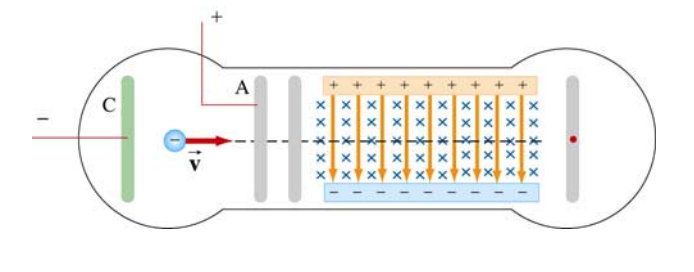
\includegraphics[scale=0.7]{apparatus}
	\caption{Particle accelerating from $C$ to $A$.}
	\label{fig:apparatus}
\end{figure}

Suppose we have electrons with charge $q = -e$ and mass $m$ emitted from the cathod $C$ and then accelerated toward slit $A$. Let the potential different between $A$ and $C$ be $V_A - V_C = \Delta V$. Given that we are selecting for particles that will travel in a straight line, find the charge to mass ($e/m$) ratio in terms of $E$, $B$, and $\Delta V$.
\subsection{Conceptual Questions} %8.10.2, 8.10.5
\textbf{Problem 2}.  If no work can be done on a charged particle by the magnetic field, how can the motion of the particle be influenced by the presence of a field?

\textbf{Problem 3}.  If a compass needle is placed in a uniform magnetic field, is there a net magnetic force acting on the needle? Is there a net torque?

\subsection{More Practice} %8.11.3, 8.11.4, 8.11.6
\textbf{Problem 4}. A conducting bar of length is placed on a frictionless inclined plane which is tilted at an angle $\theta$ from the horizontal:
\begin{figure}[h!]
	\centering
	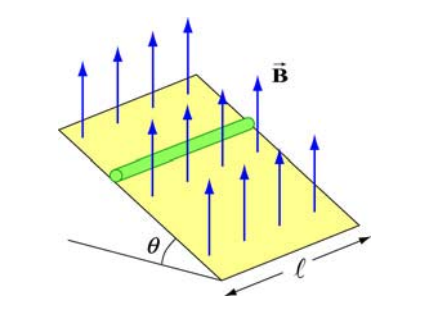
\includegraphics[scale=0.7]{sliding-bar}
	\caption{Magnetic force on a conducting bar.}
	\label{fig:bar}
\end{figure}

A uniform magnetic field is applied in the vertical direction. To prevent the bar from
sliding down, a voltage source is connected to the ends of the bar with current flowing
through. Determine the magnitude and the direction of the current such that the bar will
remain stationary.

\textbf{Problem 5}. A particle of charge -$q$ is moving with a velocity $\bv{v}$. It then enters midway between two plates where there exists a uniform magnetic field pointing into the page:
\begin{figure}[h!]
	\centering
	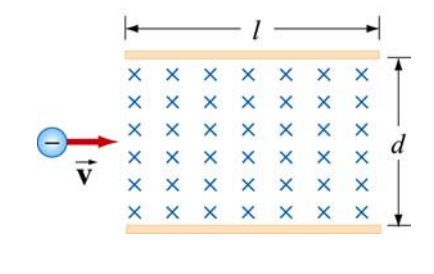
\includegraphics[scale=0.7]{particle-traj}
	\caption{Charged particle moving in magnetic field.}
	\label{fig:particle-traj}
\end{figure}
\begin{itemize}
	\item Is the trajectory of the particle deflected upwards or downwards?
	\item Compute the distance between the left end of the plate and where the particle strikes.
\end{itemize}
\newpage

\textbf{Problem 6}. A current loop consists of a semicircle of radius $R$ and two straight segments of length $l$ with an angle $\theta$ between them. The loop is then placed in a uniform magnetic field pointing to the right:
\begin{figure}[h!]
	\centering
	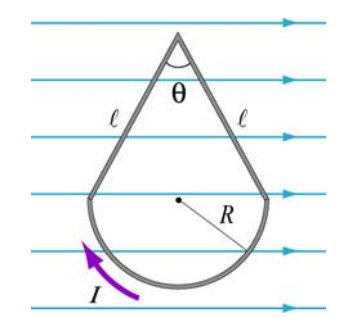
\includegraphics[scale=0.7]{weird-loop}
	\caption{Current loop in uniform magnetic field.}
	\label{fig:weird-loop}
\end{figure}
\begin{itemize}
	\item Find the net force on loop.
	\item Find the net torque on loop.
\end{itemize}

\end{document}
